\chapter{Hintergrund und Stand der Technik}

\section{Network-On-Chip (NoC)}
Ein Network-on-Chip ist ein Kommunikationssystem, das in modernen System-on-Chip (SoC) Architekturen verwendet wird, um verschiedene Komponenten (z.B. Prozessoren, Speicher und spezialisierte Einheiten) effizient miteinander zu verbinden. Statt klassische Busse oder Punkt-zu-Punkt-Verbindungen zu nutzen, setzt NoC auf ein netzwerkartiges Kommunikationsprinzip, das von Computernetzwerken oder Hochleistungsrechnern inspiriert ist. \TODO{Add References}

Die Grafik~\ref{fig:Evolution_of_Interconnection} zeigt die Entwicklung der Bus-Technologien der vergangenen Jahre.
\begin{figure}[htbp]
    \centering
    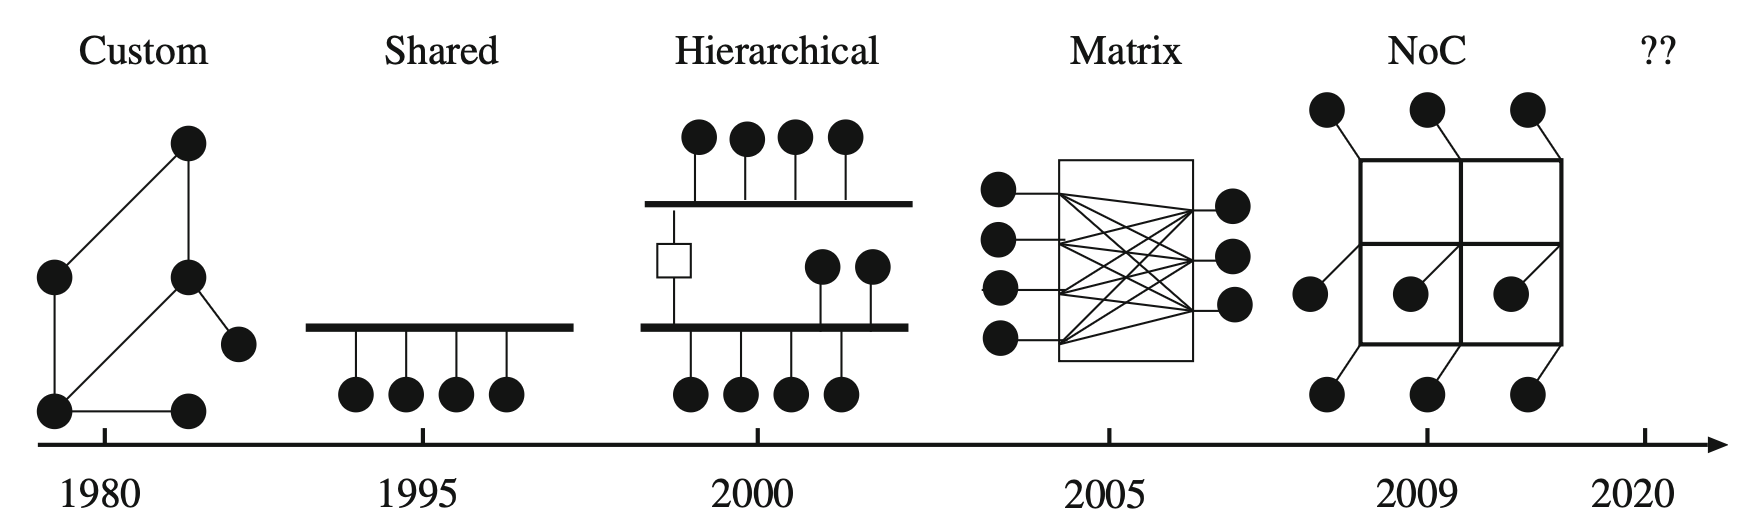
\includegraphics[width=0.95\textwidth]{img/Evolution of On-Chip communication interconnect.png}
    \caption{Evolution of Interconnections~\cite{BenAbdallah2013}}  \label{fig:Evolution_of_Interconnection}
\end{figure}

Vor 1980 wurden in der Regel maßgeschneiderte (Custom) Lösungen für die On-Chip-Kommunikation verwendet. Ab etwa 1995 kamen sogenannte Shared-Bus-Architekturen wie ARM's AMBA-Bus\TODO{ar} und IBM's CoreConnect\TODO{ar} zum Einsatz. Diese Ansätze ermöglichten ein modulareres Design mit standardisierten Schnittstellen und unterstützten die Wiederverwendung von IP-Komponenten (IP-Reuse).
Mit zunehmendem Bandbreitenbedarf stellten sich Shared-Bus-Systeme jedoch als Engpass (Bottleneck) heraus. Um dieses Problem zu umgehen, wurden hierarchische Busarchitekturen eingeführt. Diese nutzen mehrere Busse oder Bussegmente, um die Last des Hauptbusses zu verringern. Lokale Kommunikation zwischen Modulen auf demselben Bussegment ist so möglich, ohne den gesamten Bus zu belasten. Allerdings sind solche Architekturen nur begrenzt skalierbar, wenig flexibel und führen zu steigender Designkomplexität. Je mehr Kerne angeschlossen sind, desto schwieriger wird es, Timing-Vorgaben (Time Closure) und Quality-of-Service (QoS) sicherzustellen.\TODO{Begrifflichkeiten erläutern}
Eine weitere Alternative stellte die Bus-Matrix dar – ein vollständiges Crossbar-System, das parallele Verbindungen zwischen Komponenten erlaubt. Doch auch hier steigt mit zunehmender Systemgröße die Komplexität der Verdrahtung und kann schließlich den Aufwand für die Logik selbst übersteigen. Zudem trennen solche Systeme nicht klar zwischen Transport-, Transaktions- und physikalischer Schicht. Wird also ein Systemupgrade erforderlich, betrifft dies häufig das gesamte Schnittstellendesign sowie alle daran angeschlossenen Blöcke.
Vor diesem Hintergrund schlugen einige Forscher Anfang der 2000er Jahre vor, die Kommunikation zwischen verschiedenen Recheneinheiten auf einem Chip über eine vordefinierte Plattform zu realisieren – ein integriertes Schaltnetzwerk, bekannt als Network-on-Chip (NoC). NoCs erfüllen zentrale Anforderungen moderner SoCs: Wiederverwendbarkeit, skalierbare Bandbreite sowie Energieeffizienz. NoC haben die verdrahteten Verbindungen ersetzt und nutzen dafür intelligente Netzwerkinfrastrukturen. Hierbei bedient sich NoC an Modellen, Techniken und Werkzeugen der Netzwerkkommunikation, sodass festverdrahtete Kommunikation durch Paketübertragung ersetzt wird.\TODO{ar}

Ein NoC besteht aus den folgenden drei wesentlichen Komponenten:
\begin{enumerate}
    \item \textbf{Links}, die physisch die Knoten (Nodes) miteinander verbinden und die Kommunikation zwischen ihnen ermöglichen. Ein Link verbindet jeweils zwei Router (siehe Punkt 2). Ein Link kann einen oder mehrere logische Kanäle enthalten; ein Kanal wiederum besteht aus einem Satz von Leitungen (Kabeln). Die Implementierung eines Links umfasst auch die Definition des Synchronisierungsprotokolls zwischen dem Quell- und dem Zielknoten.
    \item \textbf{Router}, die für die Umsetzung des Kommunikationsprotokolls verantwortlich sind. Ein Router verfügt über mehrere Eingangs- und Ausgangsports sowie über eine Switching-Matrix, die die Verbindung zwischen diesen Ports herstellt. Zusätzlich besitzt jeder Router einen lokalen Port, der mit dem jeweiligen IP-Kern verbunden ist. Ein Logikblock innerhalb des Routers steuert die Flusskontrolle (Flow Control Policies) und legt die allgemeine Strategie für die Datenweiterleitung fest.\TODO{Flusskontrolle erklären}
    \item \textbf{Network Adapter (NA)} bzw. \textbf{Network Interface (NI)} stellen die logische Schnittstelle zwischen den IP-Kernen (IP Cores) und dem Netzwerk (NoC) dar. Sie sind notwendig, da die internen Kommunikationsmechanismen eines IP-Kerns (z.B. Busprotokolle wie AXI) typischerweise nicht direkt mit den paketbasierten Mechanismen eines NoC kompatibel sind.
\end{enumerate}

Network-on-Chip (NoC) können durch die Struktur ihrer Router-Verbindungen charakterisiert werden. Diese Struktur wird auch als \textit{Topologie} bezeichnet und typischerweise als Graph $G(N, C)$ dargestellt, wobei $N$ die Menge der Router (Nodes) und $C$ die Menge der Kanäle (Edges) repräsentiert. Man unterscheidet dabei grundsätzlich zwischen \textit{direkter} und \textit{indirekter Topologie}.
Bei der \textit{direkten Topologie} ist jedem Router genau ein Prozessor zugeordnet. Dieses Paar wird als Knoten (Node) im Netzwerk betrachtet. Jede Node ist mit einer festen Anzahl von Nachbarn verbunden, und Nachrichten werden über eine oder mehrere Zwischenknoten (Router) transportiert. Häufig verwendete Strukturen sind dabei n-dimensionale Gitter (grids), Mesh-Topologien oder Torus-Topologien (auch k-ary n-cubes genannt).
In der \textit{indirekten Topologie} sind nicht alle Router direkt mit einer Processing Unit verbunden, wie es beim direkten Modell der Fall ist. Einige Router dienen ausschließlich dazu, Nachrichten durch das Netzwerk zu routen, während andere für Steuerungs- und Verwaltungsfunktionen zuständig sind. Diese sogenannten Logikrouter fungieren dabei als Quelle (Source) oder Ziel (Target) von Nachrichten.

\TODO{Routing Algorithmen}

\TODO{Flow Control}

\TODO{Protokolldesign}

\TODO{Vor- und Nachteile}


\section{AXI4-Protokoll}

\section{QoS-Konzepte}

\section{Vergleichbare Literaturansätze}
